\documentclass[final,twoside]{rapport}  % options [chapter,final]
\usepackage{schoolbook,graphicx,paperhead,tabularx,manual,psfrag,verbatim}

\DeclareMathOperator{\E}{E}

\bibliographystyle{LongLabels}

\begin{document}

\thispagestyle{empty}
\setlength{\parindent}{0pt}
\setlength{\parskip}{1em plus 0.1em minus 0.1em}
%\addtolength{\oddsidemargin}{-1em}

\begin{paperhead}
\title{Jitterbug 1.24 Reference Manual}
\today
\author{\normalsize Anton Cervin, Bo Lincoln}
\address{Department of Automatic Control, LTH \\ Lund University \\  Box 118, SE 221 00 Lund, Sweden \\
{\tt \{anton,lincoln\}@control.lth.se}} 
\end{paperhead}

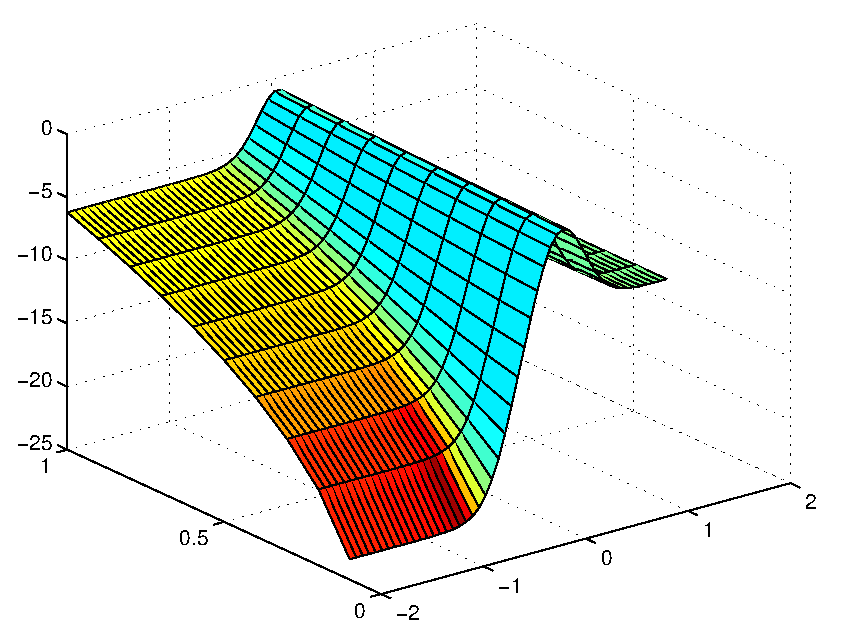
\includegraphics[width=\hsize]{cover.eps}

\newpage

\tableofcontents

\section{Introduction}

\textsc{Jitterbug} \cite{lin+02} is a \textsc{Matlab}-based toolbox
that allows the computation of a quadratic performance criterion for a
linear control system under various timing conditions. Using the
toolbox, one can easily and quickly assert how sensitive a control
system is to delay, jitter, lost samples, etc., without resorting to
simulation. The tool is quite general and can also be used to
investigate jitter-compensating controllers, aperiodic controllers,
and multi-rate controllers. As an additional feature, it is also
possible to compute the spectral density of the signals in the control
system. The main contribution of the toolbox, which is built on
well-known theory (LQG theory and jump linear systems), is to make it
easy to apply this type of stochastic analysis to a wide range of
problems.

\section{System Description}

In \textsc{Jitterbug}, a control system is described by two parallel
models: a signal model and a timing model. The signal model is
given by a number of connected, linear, continuous- and
discrete-time systems. The timing model consists of a number of
timing nodes and describes when the different discrete-time systems
should be updated during the control period.

An example of a {\sc Jitterbug} model is shown in
Figure~\ref{fig:example1},
\begin{figure}[bp]
  \centerline{
  \psfrag{H1}[c][c]{$H_1(z)$}
  \psfrag{H2}[c][c]{$H_2(z)$}
  \psfrag{H3}[c][c]{$H_3(z)$}
  \psfrag{G(s)}[c][c]{$G(s)$}
  \psfrag{y}[c][c]{$y$}
  \psfrag{u}[c][c]{$u$}
  \psfrag{v}[c][c]{$v$}
  \psfrag{e}[c][c]{$e$}
  \psfrag{n1}[c][c]{$1$}
  \psfrag{n2}[c][c]{$2$}
  \psfrag{n3}[c][c]{$3$}
  \psfrag{t1}[c][c]{$\tau_1$}
  \psfrag{t2}[c][c]{$\tau_2$}
  \psfrag{(a)}[c][c]{\small (a)}
  \psfrag{(b)}[c][c]{\small (b)}
  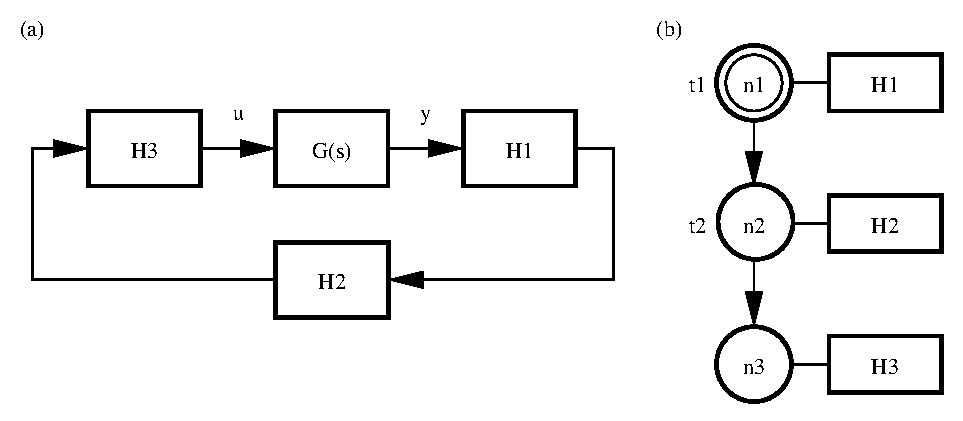
\includegraphics[scale=0.63]{example1.eps}
  }
  \caption{A simple \textsc{Jitterbug} model of a computer-controlled system:
    (a) signal model and (b) timing model.}
  \label{fig:example1}
\end{figure}
where a computer-controlled system is
modeled by four blocks. The plant is described by the continuous-time
system $G$, and the controller is described by the three discrete-time
systems $H_1$, $H_2$, and $H_3$. The system $H_1$ could represent a
periodic sampler, $H_2$ could represent the computation of 
the control signal, and $H_3$ could represent the actuator. The
associated timing model says that, at the beginning of each period,
$H_1$ should first be executed (updated). Then there is a random delay
$\tau_1$ until $H_2$ is executed, and another random delay $\tau_2$
until $H_3$ is executed. The delays could model computational delays,
scheduling delays, or network transmission delays.


\subsection{Signal Model}

The signal model consists of a number of inter-connected
continuous-time and discrete-time linear systems driven by white
noise. The cost is specified as a stationary, continuous-time
quadratic cost function.

\subsubsection{Continuous-Time Systems.}
A continuous-time system is described by
\[
\begin{aligned}
\dot x(t) &= A x(t) + B u(t-\tau) + v_c(t) \\
y^0(t) &= C x(t) \qquad\qquad  \text{(continuous output)} \\
y(t_k) &= y^0(t_k) + e(t_k) \quad \text{(sampled output with noise)}
\end{aligned}
\]
where $A$, $B$, and $C$ are constant matrices, and $v_c$ is a
continuous-time white-noise process with zero mean and covariance function
\[
\E \, v_c(t)v_c^T\!(s) = R_{1c} \, \delta(t-s),
\]
$e$ is a discrete-time
white-noise process with zero mean and covariance $R_2$, and
$\tau$ is a plant transport delay. Note that direct terms are not allowed
(i.e., the system must be strictly proper). Also note that there is no
{\em continuous-time} output noise. The ability to specify
discrete-time measurement noise in connection with the plant is only
offered as a convenience. The discrete-time output noise will be
translated to input noise at any connected discrete-time system(s).

The cost of the system is specified as
\[
J_c = \lim_{T \rightarrow \infty} \frac{1}{T} \int_0^T
  \begin{gmatrix} x(t) \\ u(t) \end{gmatrix}^{\!T} \! Q_c
  \begin{gmatrix} x(t) \\ u(t) \end{gmatrix} dt
\]
where $Q_c$ is a positive semi-definite matrix.

The system may also be specified in transfer-function form (see the
description of {\tt addcontsys} on page~\pageref{sec:addcontsys}).

\subsubsection{Discrete-Time Systems.}
A discrete-time system is described by
\[
\begin{aligned}
x(t_{k+1}) &= \Phi x(t_k) + \Gamma u (t_k) + v(t_k) \\
y^0(t_k) &= C x(t_k) + D u(t_k) \quad \text{(discrete output)}\\
y(t_k) &= y^0(t_k) + e(t_k) \qquad \;\, \text{(sampled output with noise)}
\end{aligned}
\]
where $\Phi$, $\Gamma$, $C$, and $D$ are possibly time-varying matrices (see
below). The covariance of the discrete-time white noise processes
$v$ and $e$ is given by
\[
\E \begin{gmatrix} v(t_k) \\ e(t_k) \end{gmatrix} \!\!
\begin{gmatrix} v(t_k)
  \\ e(t_k) \end{gmatrix}^{\!T} = R
\]
The update instants $t_k$ are determined by the timing model and are
not necessarily equidistant in time. The input signal $u$ is
sampled when the system is updated, and the state $x$ and the output
signal $y^0$ are held between updates.

The cost of the system is specified as  
\[
J_d = \lim_{T \rightarrow \infty} \frac{1}{T} \int_0^T
  \begin{gmatrix} x(t) \\ y^0(t) \\ u(t) \end{gmatrix}^{\!T} \! Q_d
  \begin{gmatrix} x(t) \\ y^0(t) \\ u(t) \end{gmatrix} dt
\]
where $Q_d$ is a positive semi-definite matrix. Note that $x(t)$ and
$y^0(t)$ are piecewise constant signals, while $u(t)$ may be a continuous
signal. 

The system may also be specified in transfer-function form (see the
description of {\tt   adddiscsys} on page~\pageref{sec:adddiscsys}).

\subsubsection{Connecting Systems.}
The total system is formed by appropriately connecting the
inputs and outputs of a number of continuous-time and discrete-time
systems. Throughout, MIMO formulations are allowed, and a system may
collect its inputs from a number of other systems. The total cost to
be evaluated is summed over all continuous-time and discrete-time
systems:
\begin{equation}
\label{eq:totcost}
J = \sum J_c +  \sum J_d
\end{equation}

It's important to understand how cost and noise are handled when
systems are interconnected. Three principal cases can be distinguished
(see Figure~\ref{fig:connecting}):
\begin{itemize}
\item[(a)] The interconnection of two continuous-time systems. Note that any discrete-time
  output noise $e$ will be ignored. 
\item[(b)] The interconnection of two discrete-time systems. No
  surprises here.
\item[(c)] The interconnection of a continuous-time  and a
  discrete-time system. Note that 
  the discrete-time output noise $e$ will not be included in
  the input cost of the discrete-time system.
\end{itemize}

\begin{figure}[tbp]
  \psfrag{a}[c][c]{\small (a)}
  \psfrag{b}[c][c]{\small (b)}
  \psfrag{c}[c][c]{\small (c)}
  \psfrag{u}[][]{$u$}
  \psfrag{vc}[][]{$v_c$}
  \psfrag{vd}[][]{$v$}
  \psfrag{ed}[][]{$e$}
  \psfrag{G1s}[][]{$G_1(s)$}
  \psfrag{G2s}[][]{$G_2(s)$}
  \psfrag{H1z}[][]{$H_1(z)$}
  \psfrag{H2z}[][]{$H_2(z)$}
  \psfrag{Gs}[][]{$G(s)$}
  \psfrag{Hz}[][]{$H(z)$}
  \psfrag{J}[][]{$J$}
  \psfrag{y}[][]{$y$}
  \psfrag{y0}[][]{$y^0$}
  \psfrag{e}[][]{$e$}
  \centerline{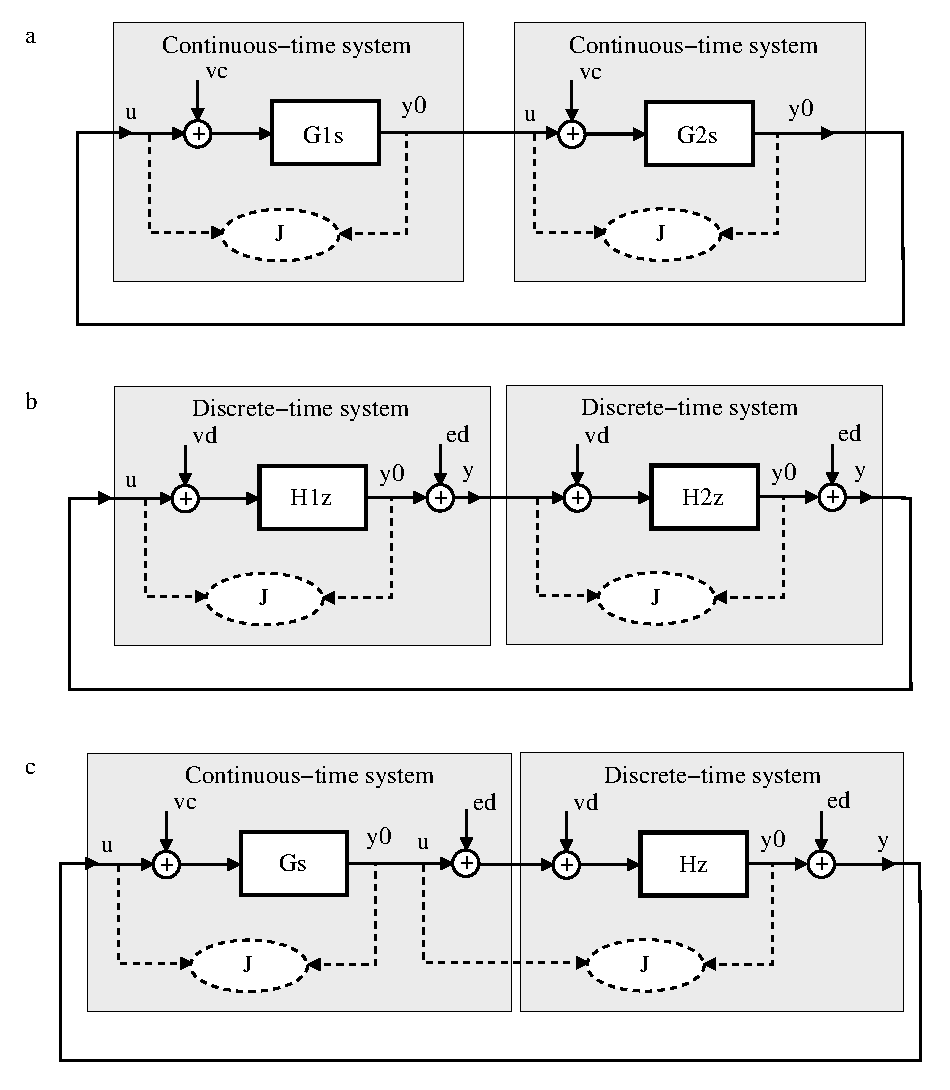
\includegraphics[width=0.9\hsize]{connecting.eps}}
  \caption{Possible interconnections of continuous-time and
    discrete-time systems.}
  \label{fig:connecting}
\end{figure}

\subsection{Timing Model}
The timing model consists of a number of timing nodes. Each node
can be associated with zero or more discrete-time systems in the
signal model, which should be updated when the node becomes active. At
time zero, the first node is activated. The first node can also be
declared to be {\em periodic} (indicated by an extra circle in the
illustrations), which means that the execution will restart at this
node every $h$ seconds. This is useful for modeling periodic
controllers and also greatly simplifies the cost calculations.

Each node is associated with a time delay $\tau$, which must elapse
before the next node can become active. (If unspecified, the delay is
assumed to be zero.) The delay can be used to model computational
delay, transmission delay in a network, etc. A delay is described by a
discrete-time probability density function
\begin{equation*}
P_\tau = \begin{bmatrix} P_\tau(0) & P_\tau(1) & P_\tau(2) & \ldots
\end{bmatrix},
\end{equation*}
where $P_\tau(k)$ represents the probability of a delay of
$k\delta$ seconds. The time grain $\delta$ is a constant that is
specified for the whole model.

In periodic systems, the execution is preempted if the total delay
$\sum \tau$ in the system exceeds the period $h$. Any remaining
timing nodes will be skipped. This models a real-time system where
hard deadlines (equal to the period) are enforced and the control task
is aborted at the deadline.

An aperiodic system can be used to model a real-time system where the
task periods are allowed to drift if there are overruns. It could also
be used to model a controller that samples ``as fast as
possible'' instead of waiting for the next period.

\subsubsection{Time-Dependent Delays.}

A delay distribution may be dependent on the time since the most
recent activation of the first node. The delay is then described by a
matrix
\begin{equation*}
P_\tau = \begin{gmatrix} P_\tau(0,\,0) & P_\tau(0,\,1) & \ldots \\
                         P_\tau(1,\,0) & P_\tau(1,\,1) & \ldots \\
                         \vdots & \vdots & \ddots\end{gmatrix},
\end{equation*}
where $P_\tau(j,\,k)$ represents the probability of a delay of $k\delta$
seconds given a previous total delay of $j\delta$ seconds.


\subsubsection*{Node- and Time-Dependent Execution.}
The same discrete-time system may be updated in several timing nodes.
It is possible to specify different update equations (i.e., different
$\Phi$, $\Gamma$, $C$ and $D$ matrices) in the various cases. This can
be used to model a filter where the update equations look different
depending on whether or not a measurement value is available. An
example of this type is given later.

It is also possible to make the update equations depend on the time
since the first node became active. This can be used to model
jitter-compensating controllers for example.

\subsubsection*{Alternative Execution Paths.}
For some systems, it is desirable to specify alternative execution
paths (and thereby multiple next nodes). In {\sc Jitterbug}, two
such cases can be modeled (see Figure~\ref{fig:altexec}):
\begin{itemize}
\item[(a)] A vector $n$ of next nodes can be specified with a
  probability vector $p$. After the delay, execution node $n(i)$ will
  be activated with probability $p(i)$. This can be used to model 
  a sample being lost with some probability.
\item[(b)] A vector $n$ of next nodes can be specified with a
  timevector $t$. If the total delay in the system since the 
  node exceeds $t(i)$, node $n(i)$ will be activated next. This can be
  used to model time-outs and various compensation schemes.
\end{itemize}

\begin{figure}[tbp]
  \centerline{
    \psfrag{n1}[c][c]{$1$}
    \psfrag{n2}[c][c]{$2$}
    \psfrag{n3}[c][c]{$3$}
    \psfrag{n4}[c][c]{$4$}
    \psfrag{t1}[c][c]{$\tau_1$}
    \psfrag{t2}[c][c]{$\tau_2$}
    \psfrag{t1<t}[c][c]{$\tau_1\!<\!t$}
    \psfrag{t1>t}[c][c]{$\tau_1\!\geq \!t$}
    \psfrag{st1<t}[c][c]{$\sum \! \tau\!<\!t$}
    \psfrag{st1>t}[c][c]{$\sum \! \tau\!\geq \!t$}
    \psfrag{p1}[c][c]{$p(2)$}
    \psfrag{p2}[c][c]{$p(3)$}
    \psfrag{(a)}[c][c]{\small (a)}
    \psfrag{(b)}[c][c]{\small (b)}
    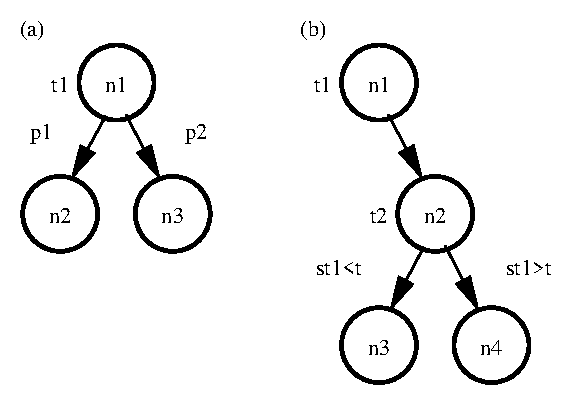
\includegraphics[scale=0.63]{altexec2.eps}
    }
  \caption{Alternative execution paths in a {\sc Jitterbug} execution
    model: (a) random choice of path and (b) choice of path depending
    on the total delay from the first node.} 
  \label{fig:altexec}
\end{figure}

\section{Internal Workings}

Inside {\sc Jitterbug}, the states and the cost are considered
in continuous time. The inherently discrete-time states, e.g. in
discrete-time controllers or filters, are treated as continuous-time
states with zero dynamics. This means that the total system can be
written as 
\begin{equation}
\label{eq:contdyn}
\dot x(t) = Ax(t) + w(t)
\end{equation}
where $x$ collects all the states in the system, and $w$ is
continuous-time white noise process with covariance matrix
$\widetilde{R}$.  To model the discrete-time changes of some states as a
timing node $n$ is activated, the state is instantaneously
transformed by
\begin{equation*}
\label{eq:discdyn}
x(t^+) = E_n x(t) + e_n(t)
\end{equation*}
where $e_{n}$ is a discrete-time white noise process with covariance $W_n$.

The total cost (\ref{eq:totcost}) for the system can be written as
\begin{equation}
\label{eq:contcost}
J =  \lim_{T\rightarrow \infty} \frac{1}{T} \int_0^T \! x^T\!(t)
  \widetilde Q
  x(t) \, dt
\end{equation}
where $\widetilde Q$ is a positive semidefinite matrix.

\subsection{Sampling the System}
{\sc Jitterbug} relies on discretized time to calculate the
 variance of the states and the cost. No approximations are involved,
 however. Sampling the
system (\ref{eq:contdyn}) with a period of $\delta$ (the time-grain
in the delay distributions) gives
\begin{equation}
\label{eq:sampleddyn}
x(k\delta+\delta) = \Phi x(k\delta) + v(k\delta)
\end{equation}
where the covariance of $v$ is $R$, and the cost (\ref{eq:contcost}) becomes
\begin{equation*}
J=\lim_{N\rightarrow \infty} \frac{1}{N\delta} 
\sum_{k=0}^{N-1} \Bigl ( x^T(k\delta) Q x(k\delta) +q \Bigr )
\end{equation*}
The matrices $\Phi$, $R$, $Q$, and $q$ are calculated as
\begin{align*}
\Phi & = e^{A\delta}\\
R &= \int_0^\delta e^{A(\delta-\tau)} \widetilde{R} e^{A^T(\delta-\tau)}~d\tau\\
Q &= \int_0^\delta e^{A^Tt} \widetilde{Q} e^{At}~dt\\
q &= {\rm tr} \Bigl ( \widetilde{Q} \int_0^\delta \int_0^\delta
e^{A(t-\tau)} \widetilde{R} e^{A^T(t-\tau)}~d\tau~dt \Bigr )
\end{align*}
or, equivalently, from
\begin{equation*}
\begin{gmatrix}
P_{11} & P_{12} \\
P_{21} & P_{22}
\end{gmatrix} \!
= \exp \left ( \begin{gmatrix}
-A^T & \widetilde{Q} \\
0 & A 
\end{gmatrix} \! \delta \right)
\end{equation*}
and
\begin{equation*}
\begin{gmatrix}
M_{11} & M_{12} & M_{13} \\
M_{21} & M_{22} & M_{23} \\
M_{31} & M_{32} & M_{33}
\end{gmatrix}\!
=\exp \left( \begin{gmatrix}
\!-A & I & 0 \\
0 & \!\!-A & \widetilde{R}^T \\
0 & 0 & A^T  
\end{gmatrix} \! \delta \right)
\end{equation*}
\vspace{-1em}
so that
\begin{align*}
\Phi & = P_{22} \\
Q & = P_{22}^T P_{12}\\
R & = M_{33}^T M_{23}\\
q & = {\rm tr} \bigl ( Q M_{33}^T M_{13} \bigr )
\end{align*}
\subsection{Timing Representation}
As time is discretized, we can transform the system description into a
jump linear system, where the Markov state represents the current timing
state of the system. Each timing node is represented by one Markov
node. In between timing nodes additional Markov nodes representing
the delay are inserted as illustrated in Figure~\ref{fig:markovjump}.

\begin{figure}[tbp]
\center
\psfrag{tau}{\small $\tau = [\, 0~\,0.1~\,0.2~\,0.3~\,0.4 \,]$}
\psfrag{p1}{\small 0.4}
\psfrag{p2}{\small 0.3}
\psfrag{p3}{\small 0.2}
\psfrag{p4}{\small 0.1}
\psfrag{1}{\small 1}
\psfrag{2}{\small 2}
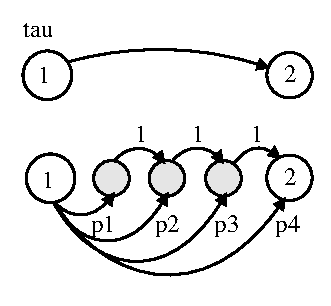
\includegraphics[scale=.8]{markovjump.ps}
\caption{A random delay (above) modeled as a jump linear system
  (below), where the delay is represented by additional Markov nodes
  in between the timing nodes.}
\label{fig:markovjump}
\end{figure}

Consider following one path in the Markov chain. For each node
which is not a timing node, only the continuous states of the
system change. In each time-step, they evolve as in
(\ref{eq:sampleddyn}), and thus the state covariance $P(k\delta) = \E \bigl \{
x(k\delta)x^T\!(k\delta) \bigr \}$ evolves as
\begin{equation*}
P(k\delta+\delta) = \Phi P(k\delta) \Phi^T + R
\end{equation*}
At each timing node $n$, the system is additionally transformed as
in (\ref{eq:discdyn}),
\begin{equation*}
P(k\delta^+) = E_n P(k\delta) E_n^T + W_n 
\end{equation*}
where $W_n$ is the covariance of the discrete-time noise $e_n(k\delta)$ in node
$n$. See Figure~\ref{fig:jumppath} for an illustration.
\begin{figure}[tbp]
\center
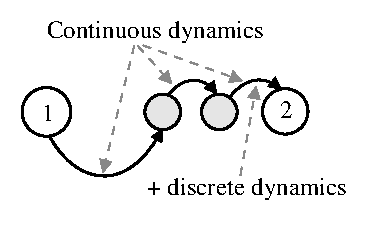
\includegraphics[scale=.8]{jumppath.ps}
\caption{The continuous-time dynamics is active between all Markov
  nodes, whereas the discrete-time dynamics is activated only before
  a timing node.}
\label{fig:jumppath}
\end{figure}
Combining the above, we define $\Phi_{n}$ as
\begin{equation*}
\Phi_{n} = \begin{cases}
\Phi & {\rm if}~n~{\rm is~not~a~timing~node}\\
E_n \Phi & {\rm if}~n~{\rm is~a~timing~node}
\end{cases}
\end{equation*}
and similarly $R_{n}$ as
\begin{equation*}
R_{n} = \begin{cases}
R & {\rm if}~n~{\rm is~not~a~timing~node}\\
E_n R E_n^T + W_n & {\rm if}~n~{\rm is~a~timing~node}
\end{cases}
\end{equation*}


\subsection{Calculating Variance and Cost}
\label{sec:calcvar}

Now consider all possible Markov states simultaneously.
Let $\pi_n(k\delta)$ be the probability of being in Markov state $n$ at time
$k\delta$, and let $P_n(k\delta)$ be the covariance of the state if the
system is in 
Markov state $n$ at time $k\delta$. Furthermore, let the transition
matrix of the Markov chain be $\sigma$, such that
\begin{equation*}
\pi(k\delta+\delta) = \sigma \pi(k\delta)
\end{equation*}
The state covariance then evolves as
\begin{equation}
\label{eq:piter}
P_n(k\delta+\delta) = \sum_{i} \sigma_{ni} \pi_i(k\delta)  
\Bigl ( \Phi_{n} P_i(k\delta) \Phi^T_{n} + R_{n} \Bigr )
\end{equation}
and the immediate cost at time $k\delta$ is calculated as
\begin{equation*}
\frac{1}{\delta} \sum_n  \pi_n(k\delta) \Bigl ({\rm tr} \bigl (
P_n(k\delta)Q \bigr ) +
q \Bigr )
\end{equation*}
For systems without a periodic node, equation (\ref{eq:piter}) must
be iterated until the cost and variance converge.
For periodic systems, the Markov state always returns to the periodic
timing node every $h/\delta$ time steps. As equation (\ref{eq:piter}) is
affine in $P$, we can find the stationary covariance $P_1(\infty)$ in
the periodic node by solving a linear system of equations.
The total cost is then calculated over the timesteps in one period.
The toolbox returns the
cost $J=\infty$ if the system is not mean-square stable.

\subsection{Calculating Spectral Densities}
For periodic systems, the toolbox also computes the discrete-time spectral
densities of all outputs as observed in the periodic timing node. The
spectral density of an output $y$ is defined as
\begin{equation*}
\phi_y(\omega) = \frac{1}{2\pi} \sum_{k=-\infty}^{\infty} \!
r_y(k) e^{-ik\omega}
\end{equation*}
The covariance function $r_y(k)$ is given by
\begin{equation*}
\begin{aligned}
r_y(k) &= \E \left\{ y(t)y^T\!(t+kh) \right\} = \E
\left\{Cx(t)x^T\!(t+kh)C^T \right\} \\
&= \E\bigl\{C\bar \Phi^{|k|} x(t)x^T\!(t)C^T\bigr\}
= C\bar \Phi^{|k|}P_1(\infty)C^T
\end{aligned}
\end{equation*}
where $\bar \Phi$ is the average transition matrix over a
period, and $P_1(\infty)$ is the stationary covariance in the periodic
node. The spectral density is returned as a discrete-time linear
system $F(z)$ such that $\phi_y(\omega) = F(e^{i\omega})$.

\section{Examples}
In this section, various examples that illustrate the use of {\sc
  Jitterbug} are given.

\subsection{Distributed Control System}

In the example, we will study the distributed control system shown in
Figure~\ref{fig:network}. The setup is taken from \cite{nilj98dis}.
\begin{figure}[htb]
  \psfrag{p1}[][] {\small \begin{tabular}{c} Actuator\\[-2mm] node \end{tabular}
}
  \psfrag{p2}[][] {\small Process}
  \psfrag{p3}[][] {\small \begin{tabular}{c} Sensor\\[-2mm] node \end{tabular}}
  \psfrag{p4}[][] {\small \begin{tabular}{c} Controller\\[-2mm] node
\end{tabular}}
  \psfrag{p5}[][] {\small Network}
  \psfrag{p6}[l][] {\small $h$}
  \psfrag{p7}[r][] {\small $\tau_1$}
  \psfrag{p8}[l][] {\small $\tau_2$}
  \psfrag{p9}[][] {}
  \psfrag{p10}[][] {\small $u(t)$}
  \psfrag{p11}[][] {\small $y(t)$}
  \centerline{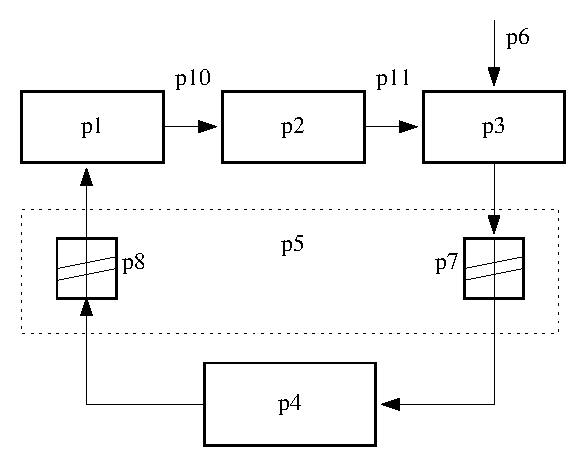
\includegraphics[width=0.5\hsize]{block.eps}}
  \caption{Distributed control system with communication
delays $\tau_1$ and~$\tau_2$.}
  \label{fig:network}
\end{figure}
In the control loop, the sensor, the actuator, and the controller are
distributed among different nodes in a network. The sensor node is
assumed to be time-driven, whereas the controller and actuator nodes
are assumed to be event-driven. At a fixed period $h$, the sensor
samples the process and sends the measurement sample over the network
to the controller node. There the controller computes a control signal
and sends it over the network to the actuator node, where it is
subsequently actuated.

The {\sc Jitterbug} model of the system was shown in
Figure~\ref{fig:example1} on page~\pageref{fig:example1}. The DC servo
process is given by the continuous-time system
\[
G(s) = \frac{1000}{s(s+1)}.
\]
The process is driven by white continuous-time input noise. There is
assumed to be no measurement noise.

The process is sampled periodically
with the interval $h$. The sampler and the actuator are described by
the trivial discrete-time systems
\[
H_1(z) = H_3(z) = 1,
\]
and the discrete-time PD controller is implemented as
\[
H_2(z) = -K \left(1+\frac{T_d}{h}\frac{z-1}{z}\right),
\]
where the controller parameters are chosen as $K=1.5$ and $T_d =
0.035$. (A real implementation would include a low-pass filter in
the derivative part, but that is ignored here.)

The delays in the computer system are modeled by the two random
variables $\tau_1$ and $\tau_2$. The total delay
from sampling to actuation is given by $\tau_{tot} = \tau_1 +
\tau_2$. It is assumed that the total delay never exceeds the sampling
period (otherwise {\sc Jitterbug} would skip the remaining updates).

As a cost function, we choose the sum of the squared
process input and the squared process output:
\begin{equation}
J = \lim_{T\rightarrow \infty} \frac{1}{T} \int_0^T \bigl ( y^2(t)
+ u^2(t) \bigr) \, dt.
\label{eq:examplecost}
\end{equation}

\subsubsection*{Sampling Period and Constant Delay.}

A control system can typically give satisfactory performance over a
range of sampling periods. In textbooks on digital control, rules of
thumb for sampling period selection are often given. One such rule
suggests that the sampling interval $h$ should be chosen such that
\[
0.2 < \omega_b h < 0.6,
\]
where $\omega_b$ is the bandwidth of the closed-loop system. In our
case, a continuous-time PD controller with the given parameters would
give a bandwidth of about $\omega_b = 80$~rad/s. This would imply a
sampling period of between 2.5 and 7.5~ms. The effect of
computational delay is typically not considered in such rules of
thumb, however. Using {\sc Jitterbug}, the combined effect of sampling
period and computational delay can be easily investigated. In
Figure~\ref{fig:perioddelay}, the cost function \eqref{eq:examplecost}
for the networked control system has been evaluated for different
sampling periods in the interval 1~to 10 milliseconds, and for
constant total delay ranging from 0~to 100\% of the sampling interval.
As can be seen, a one-sample delay gives negligible performance
degradation when $h=1$~ms. When $h=10$~ms, a one-sample delay makes
the system unstable (i.e., the cost $J$ goes to infinity).

\begin{figure}[tbp]
\center
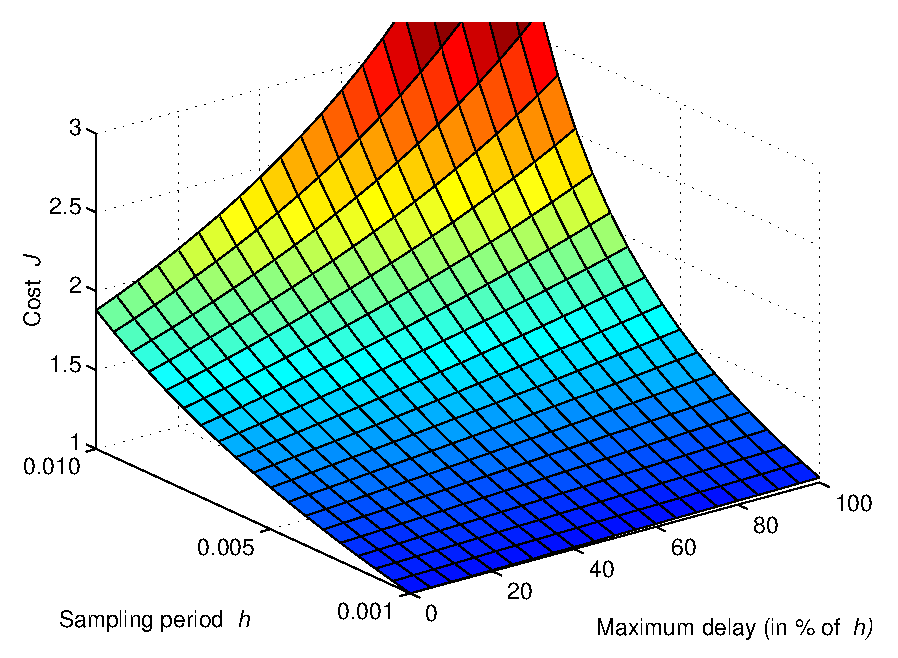
\includegraphics[width=0.75\hsize]{case2.eps}
\caption{The cost as a function of sampling period and constant delay
  in the distributed control system example.}
\label{fig:perioddelay}
\end{figure}

\subsubsection*{Random Delays and Jitter Compensation.}
If system resources are very limited (as they often are in embedded
control applications), the control engineer may have to live with long
sampling intervals. Delay in the control loop then becomes a serious
issue. Ideally, the delay should be accounted for in the control
design. In many practical cases, however, even the mean value of the
delay will be unknown at design time. The actual delay at run-time
will vary from sample to sample due to real-time scheduling, the load
of the system, etc. A simple approach is to use gain
scheduling---the actual delay is measured in each sample and the
controller parameters are adjusted according to precalculated values
that have been stored in a table. Since {\sc Jitterbug} allows
time-dependent controller parameters, such delay compensation schemes
can also be analyzed using the tool.

In the {\sc Jitterbug} model of the networked control system, we now
assume that the delays $\tau_1$ and $\tau_2$ are uniformly distributed
random variables between 0 and $\tau_{max}/2$, where
$\tau_{max}$ denotes the maximum round-trip delay in the 
loop. A range of PD controller parameters (ranging from $K=1.5$ and
$T_d=0.035$ for zero delay to $K=0.78$ and $T_d=0.052$ for
7.5~ms delay) are derived and stored in a table. When a sample
arrives at the controller node, only the delay $\tau_1$ from sensor to
controller is known, however, so the remaining delay is predicted by
its expected value of $\tau_{max}/4$. 


\begin{figure}[tbp]
\center
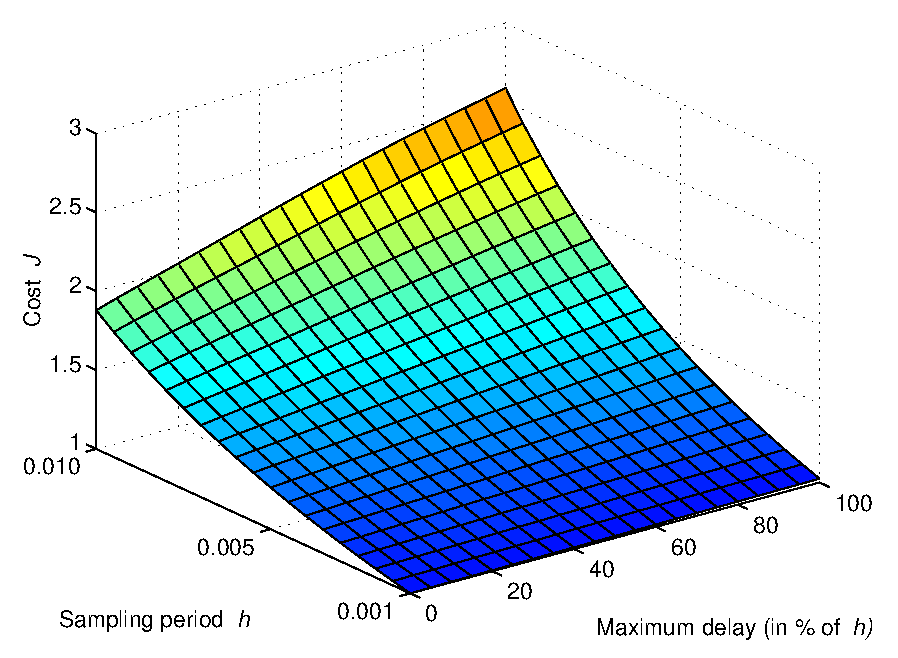
\includegraphics[width=0.75\hsize]{case6.eps}
\caption{The cost as a function of sampling period and maximum delay
  with jitter compensation in the distributed control system example.}
\label{fig:periodjitter}
\end{figure}

In Figure~\ref{fig:periodjitter}, the cost function
\eqref{eq:examplecost} for the networked control system has been
evaluated for different sampling periods in the interval 1~to 10
milliseconds, and for maximum total delay ranging from 0~to 100\% of
the sampling interval. Compared to Fig~\ref{fig:perioddelay}, the cost
is considerably lower.

The Matlab script for the computations is given below:
\begin{small}
\verbatiminput{../examples/distributed.m}
\end{small}

\subsection{Notch Filter}

Cleaning signals from disturbances using e.g. notch filters is
important in many applications. In some cases these filters are very
sensitive to lost samples due to the very narrow-band characteristics,
and in real-time systems lost samples are sometimes inevitable. In
this example {\sc Jitterbug} is used to evaluate the effects of this
problem on different filters.

The setup is as follows. A good signal $x$ (modeled as low-pass
filtered noise) is to be cleaned from an additive disturbance $e$
(modeled as band-pass filtered noise). 
An estimate $\hat x$ of the good signal should be
found by applying a digital notch filter with the sampling interval
$h=0.1$ to the measured signal $x+e$. Unfortunately, a fraction $p$ of
the measurements are lost.

A {\sc Jitterbug} model of the system is shown in
Figure~\ref{fig:timing2}.
\begin{figure}[tbp]
\centerline{
\psfrag{v1}[c][c]{$v_1$}
\psfrag{v2}[c][c]{$v_2$}
\psfrag{e}[c][c]{$e$}
\psfrag{x}[c][c]{$x$}
\psfrag{xh}[c][c]{$\hat x$}
\psfrag{xt}[c][c]{$\tilde x$}
\psfrag{G1}[c][c]{$G_1(s)$}
\psfrag{G2}[c][c]{$G_2(s)$}
\psfrag{Samp}[c][c]{\small\em Samp}
\psfrag{Diff}[c][c]{\small\em Diff}
\psfrag{Hold}[c][c]{\small\em Delay}
\psfrag{Filt(i)}[c][c]{\small\em Filter($i$)}
\psfrag{n1}[c][c]{$1$}
\psfrag{n2}[c][c]{$2$}
\psfrag{n3}[c][c]{$3$}
\psfrag{n4}[c][c]{$4$}
\psfrag{n5}[c][c]{$5$}
\psfrag{p1}[c][c]{$1\!-\!p$}
\psfrag{p2}[c][c]{$p$}
\psfrag{Filt(1)}[c][c]{\small $\mathit{Filter}(1)$}
\psfrag{Filt(2)}[c][c]{\small $\mathit{Filter}(2)$}
\psfrag{(a)}[c][c]{\small (a)}
\psfrag{(b)}[c][c]{\small (b)}
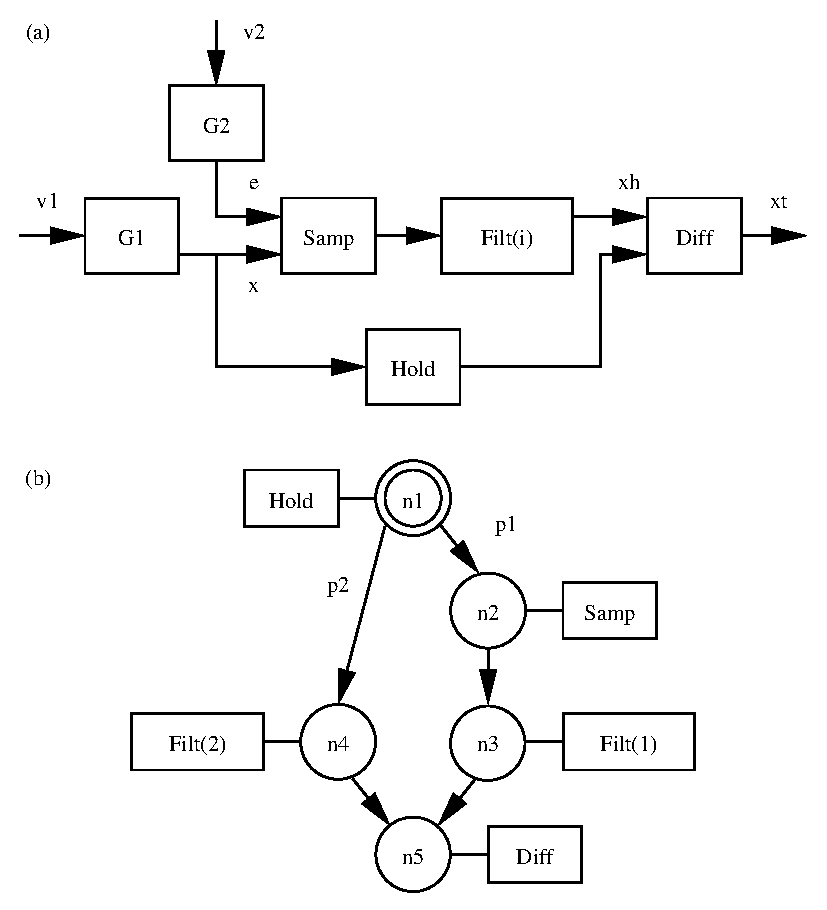
\includegraphics[scale=0.63]{example2.eps}
}
  \caption{{\sc Jitterbug} model of the notch filter: (a) signal
    model and (b) timing model.}
  \label{fig:timing2}
\end{figure}
The signals $x$ and $e$ are generated by white noise being filtered through
the continuous-time systems $G_1$ and $G_2$. 
The digital filter is represented as two discrete-time systems: {\em Samp}
and {\em Filter}. The good signal is buffered in the system {\em
  Delay} and is compared to the filtered estimate in the system {\em Diff}.
In the timing model, there is a probability $p$ that the {\em Samp}
system will not be updated. In that case, it is possible to execute an
alternate version, $\mathit{Filter}(2)$, of the filter dynamics.

Two different filters are compared. The first filter is an ordinary
second-order notch filter with two zeros on the unit circle. The same
update equations are used regardless if a sample is available or
not. The second filter is a second-order Kalman filter based on a
simple model of the signal dynamics. In the case of lost samples,
only prediction is performed in the filter.

The spectral density of the estimation error $\tilde x = x - \hat x$ in
the two filter cases is shown in Figure~\ref{fig:notchplot}. It has
been assumed that $p=10\%$ of the samples are lost. It is seen that 
the ordinary notch filter performs well around the disturbance frequency
while the lost samples introduce a large error at lower frequencies. The
time-varying Kalman filter is less sensitive towards lost samples and
has a more even error spectrum. Overall, the variance of the
estimation error is about 40\% lower in the Kalman filter case.

\begin{figure}[tbp]
\centerline{
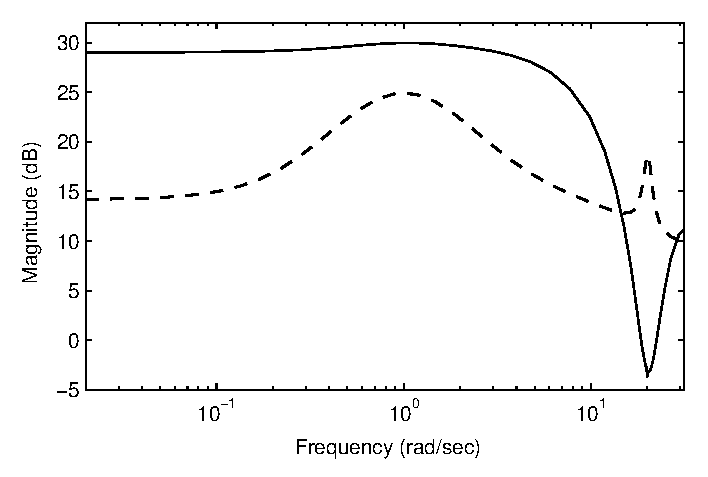
\includegraphics[scale=0.7]{fig2.eps}}
  \caption{The spectral density of the error output $\tilde x$ when 10\%
    of the samples are lost, using a notch filter (full) or a
    time-varying Kalman filter (dashed).}
  \label{fig:notchplot}
\end{figure}

The Matlab script for the computations is given below:
\begin{small}
\verbatiminput{../examples/notch.m}
\end{small}

\subsection{Multirate Controller}
In this example we will show how to compute the performance of a
multirate controller. This is illustrated on a cascade controller for
the ball and beam process, see Figure~\ref{fig:cascade}.
\begin{figure}[tbp]
\psfrag{p1}[][]{PID1}
\psfrag{p2}[][]{PID2}
\psfrag{p3}[][]{$G_\phi(s)$}
\psfrag{p4}[][]{$G_x(s)$}
\psfrag{p5}[][]{\small Controller}
\psfrag{p6}[][]{\small Process}
\psfrag{v}[][]{$v$}
\psfrag{phi}[][]{$\phi$}
\psfrag{x}[][]{$x$}
\psfrag{s}[][]{\small $\Sigma$}
\centerline{
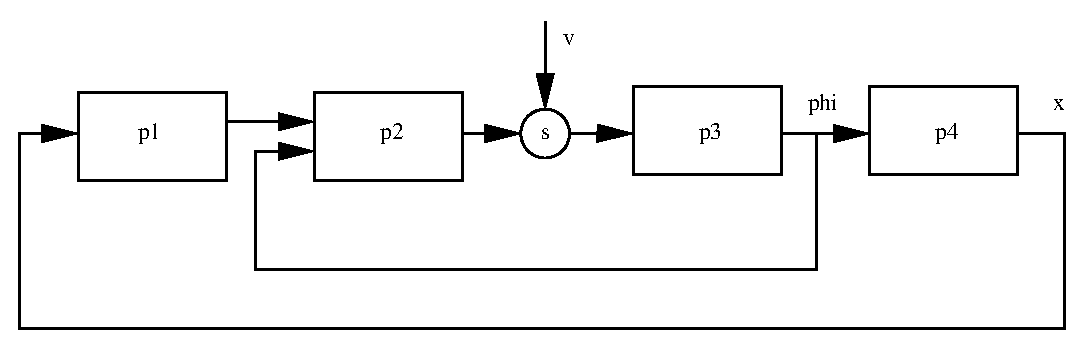
\includegraphics[scale=0.6]{cascade.eps}}
  \caption{The ball \& beam cascaded controller.}
  \label{fig:cascade}
\end{figure}
In this control structure, the inner controller, PID2, is
responsible for controlling the beam 
dynamics,
\[
G_\phi(s) = \frac{4.4}{s},
\]
while the outer controller, PID1, controls the ball on beam dynamics,
\[
G_x(s) = -\frac{9.0}{s^2}.
\]
Since the inner loop is typically designed to be much faster than the
outer loop, it can be a good idea to execute the inner loop at a
higher frequency, especially if CPU resources are scarce. We will
compare the performance of an ordinary cascade controller with a
multirate cascade controller where the inner controller executes at
twice the frequency of the outer controller.

The {\sc Jitterbug} timing model in the multirate case is shown in
Figure~\ref{fig:multiratetiming}.
\begin{figure}[bp]
  \centerline{
  \psfrag{H1}[c][c]{PID1}
  \psfrag{H2}[c][c]{PID2}
  \psfrag{H3}[c][c]{PID2}
  \psfrag{n1}[c][c]{$1$}
  \psfrag{n2}[c][c]{$2$}
  \psfrag{n3}[c][c]{$3$}
  \psfrag{t1}[r][c]{$0$}
  \psfrag{t2}[r][c]{$h/2$}
  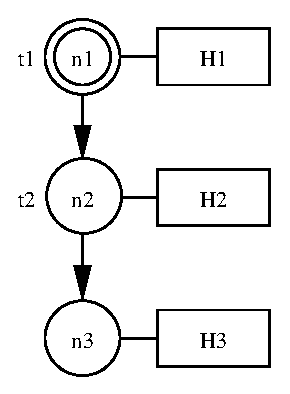
\includegraphics[scale=0.63]{multiratetiming.eps}
  }
  \caption{Timing model for the multirate ball \& beam controller.}
  \label{fig:multiratetiming}
\end{figure}
The sampling interval of the outer controller is denoted $h$. The
sampling interval of the inner controller is thus $h/2$. The execution
time of the control algorithm is ignored in this simple model. At the
beginning of each period, PID1 is executed, immediately followed by
PID2, which uses the control signal produced by PID1 as a reference
value. Then, half a period later, the PID2 is executed again, using
the same reference value as in the first invocation but a new
measurement value.

Assume that the process is disturbed by white input noise $v$ with
unit variance, and that the performance is measured by the cost
function
\[
J = \lim_{T \rightarrow \infty} \frac{1}{T} \int_0^T \! \left(
  \phi^2(t) + x^2(t) \right) dt
\]
Assuming certain PID parameters, the performance in the different
cases becomes
\[
J_\mathit{ordinary} = 3.40, \qquad J_\mathit{multirate} = 1.99.
\]
(Running both controllers at the fast rate gives $J=1.93$, i.e. only a
small further improvement.)

The Matlab script comparing the two cases is shown below:
\begin{small}
\verbatiminput{../examples/multirate.m}
\end{small}


\subsection{Spectral Density Calculation}
The following example computes the influence of jitter on the
sensitivity function for a control system. The sensitivity function
for a control system with a plant $G$ and a controller $C$ is defined
as $S = \frac{1}{1+CG}$. For a randomly time-varying system, though,
this definition cannot be used.

The idea in this example is to form a
system which is driven by white noise $e$ at the output of the process
$G$ (see Figure~\ref{fig:blockspectdens}). The spectral density of the
output $y$ may then be interpreted as a kind of sensitivity function for the
stochastic system.

\begin{figure}
  \center
  \psfrag{C}[c][c]{$C(z)$}
  \psfrag{G}[c][c]{$G(s)$}
  \psfrag{Samp}[c][c]{\small Samp}
  \psfrag{v}[c][c]{$e$}
  \psfrag{y}[c][c]{$y$}
  \psfrag{-1}[c][c]{$-1$}
  \psfrag{s}[c][c]{$\Sigma$}
  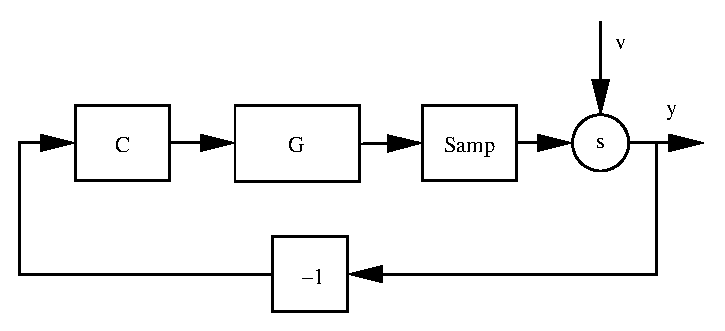
\includegraphics[width=0.6\hsize]{blockspectdens.eps}
  \caption{The signal model to calculate the sensitivity spectral
    density (i.e., the spectral density of $y$ when $e$ is
    white noise).}
  \label{fig:blockspectdens}
\end{figure}

The example system is a continuous $G(s) = \frac{1}{s^2}$ which is
controlled by a LQG-designed controller $C(z)$. The process is sampled
periodically, but there is a random delay $\tau$ between the process and the
controller (see Figure~\ref{fig:timingspectdens}).  The delay is
uniformly distributed between zero and $\tau_{\rm max}$. The
sensitivity spectral density for $\tau_{\rm max}$ between zero and $h$
(for different amounts of jitter) is plotted in
Figure~\ref{fig:spectdens}.

\begin{figure}
  \center
  \psfrag{C}[c][c]{$C(z)$}
  \psfrag{Samp}[c][c]{\small Samp}
  \psfrag{n1}[c][c]{$1$}
  \psfrag{n2}[c][c]{$2$}
  \psfrag{t1}[c][c]{$\tau$}
  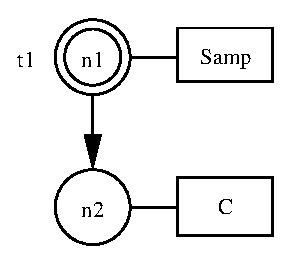
\includegraphics[scale=0.63]{timingspectdens.eps}
  \caption{The timing model of the spectral density example.}
  \label{fig:timingspectdens}
\end{figure}

\begin{figure}
  \center
  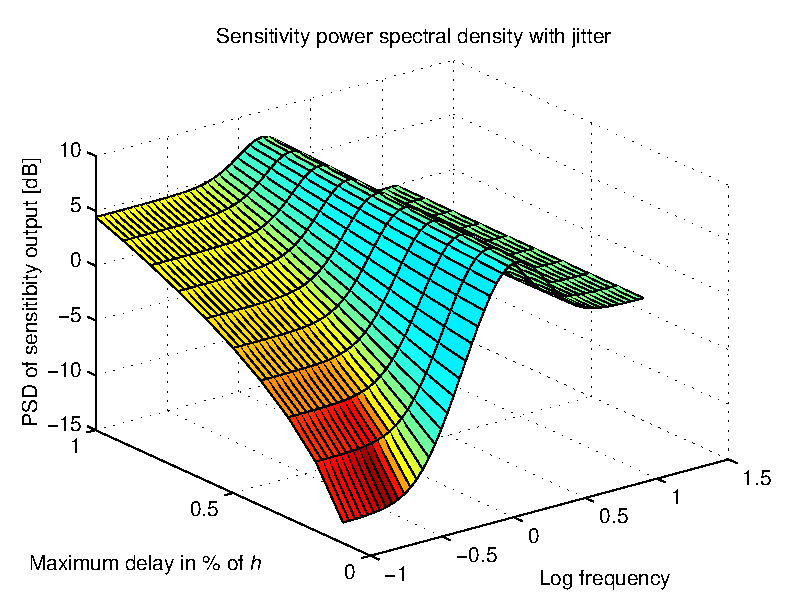
\includegraphics[width=10cm]{spectdens.eps}
  \caption{The sensitivity spectral density from the example.}
  \label{fig:spectdens}
\end{figure}

The Matlab script for the computations is given below:
\begin{small}
\verbatiminput{../examples/spectdens.m}
\end{small}

\subsection{Overrun Handling Methods}
This example presentes (a rather long) script that compares three ways
of handling long delays in a control system. The problem is what to do
if the controller does not get a process sample in time. Three
approaches are tested:
\begin{itemize}
  \item[a)] Do not update the controller, and use the old control signal.
  \item[b)] Update the controller state and control signal based on no
    input. This is not done by feeding zeros to the observer, but
    rather by disconnecting the input part of the observer. 
  \item[c)] Extend the sample period until the sample does arrive.
    This creates an aperiodic system, and an iterative solver
    has to be used.
\end{itemize}
This kind of problem can also be interpreted as a computation time
problem, where the computation of some control signal may take long
enough time to miss a deadline.

The set-up is as follows. A plant $G(s) = \frac{1}{s(s^2+2\zeta
  \omega s+\omega^2)}$ with $\zeta = 
0.2$ and $\omega=1$ is to be controlled by an LQG regulator. The
controller is calculated for the mean time
delay using the function {\tt lqgdesign()}. 
As for the delay, it is uniformly distributed between 0 and
$\tau_{\rm max}$, where $\tau_{\rm max}$ is swept from 0 to 2h (i.e.
two sample periods).

The three cases are compared in Figure~\ref{fig:overrun}. As expected,
using the old control signal gives the worst performance, while
extending the control period until the control signal is produced
gives the best results.

\begin{figure}
  \center
  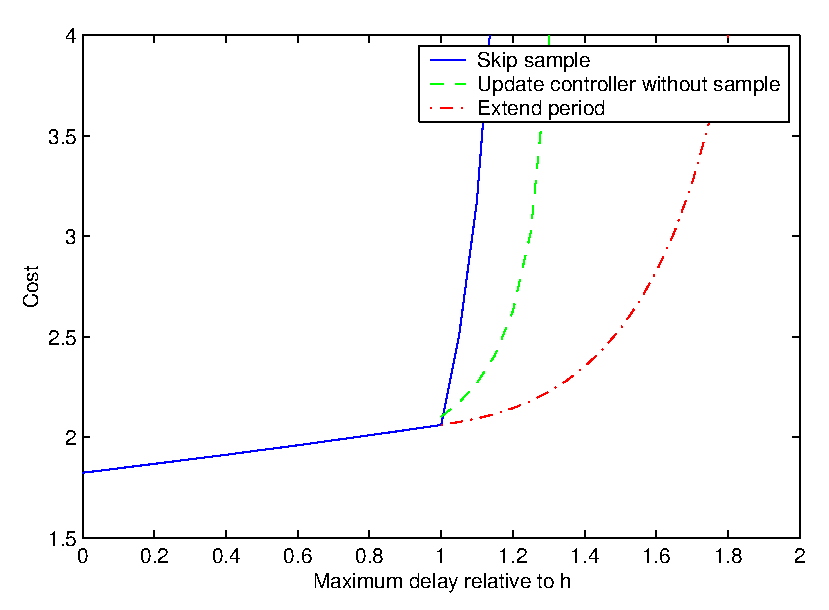
\includegraphics[width=10cm]{overrun.eps}
  \caption{The costs in the overrun example.}
  \label{fig:overrun}
\end{figure}

The Matlab script for the computations is given below. 
Note that the iterative solver is very much slower than the algebraic
solver, and is only used when the system is aperiodic.

\begin{small}
\verbatiminput{../examples/overrun.m}
\end{small}


%%%%%%%%%%%%%%%%%%%%%%%%%%%%%%%%%%%%%%%%%%%%%%%%%%%%%%%%%%%%%%%%%%%%%%

\section{Command Reference}

A summary of the available {\sc Jitterbug} commands are given in
Table~1.

\begin{table}[htbp]
\label{table:commands}
\begin{center}
\begin{tabularx}{\hsize}{|l|>{\raggedright\arraybackslash}X|}
\hline
Command & Description \\ \hline
{\tt initjitterbug} & Initialize a new {\sc Jitterbug} system. \\
{\tt addtimingnode} & Add a timing node. \\
{\tt addcontsys} & Add a continuous-time system. \\
{\tt adddiscsys} & Add a discrete-time system to a timing node. \\
{\tt adddiscexec} & Add an execution of a previously defined
discrete-time system. \\
{\tt adddisctimedep} & Add time-dependence to a previously defined
discrete-time system. \\
{\tt calcc2d} & Internal function used to sample continuous-time
dynamics, cost, and noise\\ 
{\tt calcdynamics} & Calculate the internal dynamics of a {\sc Jitterbug} system. \\
{\tt calccost} & Calculate the total cost of a {\sc Jitterbug} system
and, for periodic systems, calculate the spectral densities of the outputs. \\
{\tt lqgdesign} & Design a discrete-time LQG controller for 
a continuous-time plant with a constant or random time delay and a
continuous-time cost function.\\ \hline
\end{tabularx}
\end{center}
\caption{Summary of the {\sc Jitterbug} commands.}
\end{table}



%%%%%%%%%%%%%%%%%%%%%%%%%%%%%%%%%%%%%%%%%%%%%%%%%%%%%%%%%%%%%%%%%%%%%%

\entry{initjitterbug}
\label{sec:initjitterbug}

\purpose
Initialize a new {\sc Jitterbug} system.

\syntax
\begin{verbatim}
N = initjitterbug(delta,h)
\end{verbatim}

\descr 
Initialize a new {\sc Jitterbug} system with a given time-grain and
period.

\args
\begin{tabularx}{\hsize}{l>{\raggedright\arraybackslash}X}
  {\tt delta} & The time grain (in seconds). The computations in {\sc
    Jitterbug} are completely based on this discretization.
  Computation times and memory scale inversely proportionally to {\tt
    delta}. \\ 
  {\tt h} & The period of the system (in seconds). Specify 0 if the
  system should be aperiodic.
\end{tabularx}
 
\retvals
\begin{tabularx}{\hsize}{l>{\raggedright\arraybackslash}X}
{\tt N} & The {\sc Jitterbug} system which must be passed to all other
functions.
\end{tabularx}


%%%%%%%%%%%%%%%%%%%%%%%%%%%%%%%%%%%%%%%%%%%%%%%%%%%%%%%%%%%%%%%%%%%%%%

\entry{addtimingnode}
\label{sec:addtimingnode}

\purpose
Add a timing node to a {\sc Jitterbug} system.

\syntax
\begin{verbatim}
N = addtimingnode(N,nodeid)
N = addtimingnode(N,nodeid,Ptau,nextnode)
N = addtimingnode(N,nodeid,Ptau,nextnodes,nextprobs)
N = addtimingnode(N,nodeid,Ptau,timedepnextnodes)
\end{verbatim}

\descr
Add a timing node to the {\sc Jitterbug} system {\tt N}. The delay in
the node is given by the discrete probability distribution {\tt Ptau}.
The next node to be visited can be either deterministic, random, or
dependent on the total delay since the first node.

{\em Note 1:} The {\sc Jitterbug} system must have a node with ID 1.
If the system is periodic, this will be the periodic node.

{\em Note 2:} If the total delay exceeds the period, the execution
          will restart in the periodic node (if the system is periodic).
 
\args
\begin{tabularx}{\hsize}{l>{\raggedright\arraybackslash}X}
  {\tt N}   &  The {\sc Jitterbug} system to add this timing node to.\\
  {\tt nodeid} &   The ID of this timing node (a positive integer).\\
  {\tt Ptau} & The delay probability vector. {\tt Ptau(1)} is the
  probability of a delay of {\tt 0*delta} seconds, {\tt Ptau(2)} is
  the probability of a delay of {\tt 1*delta} seconds, etc. If
  omitted, the system will stay in this node until the next period.
  If {\tt Ptau} is a matrix, each row {\tt j} specifies the delay
  probability vector given a previous total delay of {\tt j*delta} seconds.
 \\
  {\tt nextnode} & 
  The next node to be visisited, after the delay in this node has
  elapsed. \\
  {\tt nextnodes} & A vector of possible next nodes to be visited.\\
  {\tt nextprobs} & A vector specifying the probabilities for each of
  the nodes in {\tt nextnodes} to be visited next.\\
  {\tt timedepnextnodes} & A vector of next nodes to be visited
  depending on the total delay since the first node (including the
  delay in this node).
\end{tabularx}

%%%%%%%%%%%%%%%%%%%%%%%%%%%%%%%%%%%%%%%%%%%%%%%%%%%%%%%%%%%%%%%%%%%%%%

\entry{addcontsys}
\label{sec:addcontsys}

\purpose
Add a continuous-time system to a {\sc Jitterbug} system.

\syntax
\begin{verbatim}
N = addcontsys(N,sysid,sys,inputid,Qc,R1c,R2,impulse)
\end{verbatim}

\descr
The continuous-time system can be given in state-space form or
in transfer-function (or zero-pole-gain) form.

In {\em state-space form}, the system is described by
\[
\begin{aligned}
\dot x(t) &= A x(t) + B u(t-\tau) + v_c(t) \\
y^0(t) &= C x(t) \qquad\qquad\;\,  \text{(continuous output)} \\
y(t_k) &= y^0(t_k) + e(t_k) \quad \text{(sampled output with noise)}
\end{aligned}
\]
where $v$ is a continuous-time white-noise process with zero
mean and covariance function
\[
\E \, v_c(t)v_c^T\!(s) = R_{1c} \, \delta(t-s)
\]
$e$ is a discrete-time white-noise process with zero mean and covariance $R_2$,
and $\tau$ is a constant plant transport delay. The cost of the system is
specified as
\[
J = \lim_{T \rightarrow \infty} \frac{1}{T} \int_0^T
  \begin{gmatrix} x(t) \\ u(t) \end{gmatrix}^{\!T} \! Q_c \begin{gmatrix} x(t)
    \\ u(t) \end{gmatrix} dt
\]
where $Q_c$ is a positive semi-definite matrix.

In {\em transfer-function form}, the system is described by
\[
\begin{aligned}
y^0(t) &= G(p) \Bigl( u(t-\tau) + v_c(t) \Bigr) \quad  \text{(continuous output)} \\
y(t_k) &= y^0(t_k) + e(t_k) \qquad\qquad\quad \text{(sampled output with noise)}
\end{aligned}
\]
where $G(p)$ is a strictly proper transfer function, $v$ is a
continuous-time white-noise process with zero mean and
covariance function
\[
\E \, v_c(t)v_c^T\!(s) = R_{1c} \, \delta(t-s),
\]
$e$ is a discrete-time white-noise process with
zero mean and covariance $R_2$, and $L$ is a constant plant transport
delay. The cost of the system is specified as
\[
J = \lim_{T \rightarrow \infty} \frac{1}{T} \int_0^T
  \begin{gmatrix} y^0(t) \\ u(t) \end{gmatrix}^{\!T} \!Q_c \begin{gmatrix} y^0(t)
    \\ u(t) \end{gmatrix} dt
\]
where $Q_c$ is a positive semi-definite matrix.

Note that the measured discrete output is only used when the system is
connected to a discrete-time system.

\args
\begin{tabularx}{\hsize}{l>{\raggedright\arraybackslash}X}
{\tt N} & The {\sc Jitterbug} system to add this continuous-time system to.
\\
{\tt sysid} &  A unique ID number for this system (pick any). Used when
referred to from other systems.\\
{\tt sys} & A strictly proper continuous-time LTI system in
state-space, transfer function, or pole-zero-gain form. A plant
transport delay can be specified using any of the LTI delay
attributes. The delay must be a multiple of the time-grain {\tt delta}.
\\
{\tt inputid} & A vector of system IDs. The outputs of the corresponding
systems will be used as inputs to this system. The number of inputs in
this system must equal the total number of outputs in the input
systems.  A negative input ID
          specifies that the corresponding system's {\em state} should
          be used instead of its output. An input ID of zero
          specifies that the input should be taken from the {\em null}
          system (which has a scalar output equal to zero).
\end{tabularx}

\optargs
\begin{tabularx}{\hsize}{l>{\raggedright\arraybackslash}X}
{\tt Qc} & The cost matrix (default is zero).
\\
{\tt R1c} & The state or input noise covariance matrix (default is
zero).
\\
{\tt R2} & The discrete measurement noise covariance matrix (default is zero). 
Note that measurement noise will only be added when the system is
sampled by a discrete-time system. The measurement noise {\em will
  not} be included in the input cost of the connected discrete-time
system. Also, the measurement nosie {\em will  not} affect any connected
{\em  continuous-time} systems (see Figure~\ref{fig:connecting}).\\
{\tt impulse} & If non-zero, then impulse control inputs are assumed instead of
zero-order hold inputs. This option is only possible if the input system is a
discrete-time system. The input $u(t)$ is given by
\[
u(t) = \sum_{k} u_k \delta(t-t_k)
\]
where $u_k$ is the output of the preceeding discrete-time system.
The cost of the system is modified to
\[
J = \lim_{T \rightarrow \infty} \frac{1}{T} \int_0^T
  x^T(t) Q_{1c} x(t)
     dt + \lim_{N\to\infty}\frac{1}{Nh} \sum_{k=1}^N u^T_k Q_{2c} u_k
\]
\end{tabularx}

Any optional arguments can be left as {\tt []} for default values.

\remark
Internally, the system is represented in state-space
form. A continuous-time system with $n$ states, $r$ inputs, and a
transport delay of $L$ seconds requires $n + rL/\delta$ states in the
internal description, where $\delta$ is the time-grain of the {\sc
  Jitterbug} model. A warning will be issued if $L/\delta$ is not an
integer.

\limitations
To avoid problems with algebraic loops and infinite variances, 
continuous-time systems with direct terms are not supported. Also,
continuous-time output noise is not supported.

%%%%%%%%%%%%%%%%%%%%%%%%%%%%%%%%%%%%%%%%%%%%%%%%%%%%%%%%%%%%%%%%%%%%%%


\entry{adddiscsys}
\label{sec:adddiscsys}

\purpose
 Add a discrete-time system to a {\sc Jitterbug} system.

\syntax
\begin{verbatim}
N = adddiscsys(N,sysid,sys,inputid,nodeid,Q,R)
\end{verbatim}

\descr
The discrete-time system can be given in state-space form or in
transfer-function form.

In {\em state-space form}, the system is described by
\[
\begin{aligned}
x(t_{k+1}) &= A x(t_k) + B u (t_k) + v(t_k) \\
y^0(t_k) &= C x(t_k) + D u(t_k) \quad \text{(discrete output)}\\
y(t_k) &= y^0(t_k) + e(t_k) \qquad \; \text{(sampled output with noise)}
\end{aligned}
\]
where $v$ and $e$ are discrete-time white-noise processs with zero
mean and covariance
\[
R = \E \begin{gmatrix} v(t_k) \\ e(t_k) \end{gmatrix} \!\!
\begin{gmatrix} v(t_k)
  \\ e(t_k) \end{gmatrix}^{\!T}.
\]
The cost of the system is specified as 
\[
J = \lim_{T \rightarrow \infty} \frac{1}{T} \int_0^T
  \begin{gmatrix} x(t) \\ y^0(t) \\ u(t) \end{gmatrix}^{\!T} \! Q
  \begin{gmatrix} x(t) \\ y^0(t) \\ u(t) \end{gmatrix} dt
\]
where $Q$ is a positive semi-definite matrix. Note that $x(t)$ and $y^0(t)$
are piecewise constant signals, while $u(t)$ may be a continuous signal.

In {\em transfer-function form}, the system is described by
\[
\begin{aligned}
y^0(t_k) &= H(q) \bigl( u(t_k) + v(t_k) \bigr) \quad \text{(discrete
  output)}\\
y(t_k) &= y^0(t_k) + e(t_k) \qquad\quad\;\;\; \text{(sampled output with noise)}
\end{aligned}
\]
where $H(q)$ is a proper transfer function, and
$v$ and $e$ are discrete-time white-noise processs with zero
mean and covariance 
\[
R = \E \begin{gmatrix} v(t_k) \\ e(t_k) \end{gmatrix} \!\!
\begin{gmatrix} v(t_k)
  \\ e(t_k) \end{gmatrix}^{\!T}.
\]
As an alternative, one may specify only the input noise:
\[
R = \E v(t_k)v(t_k)^{\!T}
\]
It is then assumed that $\E e(t_k)e(t_k)^{\!T} =0$.

The cost of the system is specified as 
\[
J = \lim_{T \rightarrow \infty} \frac{1}{T} \int_0^T
  \begin{gmatrix} y^0(t) \\ u(t) \end{gmatrix}^{\!T} \!Q \begin{gmatrix}
    y^0(t) \\ u(t) \end{gmatrix} dt
\]
where $Q$ is a positive semi-definite matrix. Again, note that
$y^0(t)$ is a piecewise constant signal, while $u(t)$ may be a
continuous signal.

\args
\begin{tabularx}{\hsize}{l>{\raggedright\arraybackslash}X}
{\tt  N} &  The {\sc Jitterbug} system to add this discrete-time system to.\\
{\tt sysid} &  A unique ID number of this system (pick any). Used when
referred to from other systems. \\
{\tt sys} & A discrete-time LTI system in state-space or transfer
function form, or a double/matrix (interpreted as a static gain
transfer function).\\
{\tt inputid} & A vector of system IDs. The outputs of the
corresponding systems will be used as inputs to this system. The
number of inputs in this system must equal the total number of outputs
in the input systems. A negative input ID
          specifies that the corresponding system's {\em state} should
          be used instead of its output. An input ID of zero
          specifies that the input should be taken from the {\em null}
          system (which has a scalar output equal to zero). \\
{\tt nodeid} & The timing node where this discrete-time system should
be executed. If you want the same system to be executed in further
nodes, use {\tt adddiscexec}.
\end{tabularx}

\optargs
\begin{tabularx}{\hsize}{l>{\raggedright\arraybackslash}X}
{\tt Q} & The cost matrix (default is zero). \\
{\tt R} & The noise covariance matrix (default is zero). Added each
time the system is updated. Note that noise may also enter the system
from the output nose of another system. 
\end{tabularx}

Any optional arguments can be left as {\tt []} for default values.

\remark
Internally, the system is represented in state-space
form. A discrete-time system with $n$ states and $p$ outputs requires
$n+p$ states in the internal description. (The extra states are needed
to store the zero-order hold outputs.)

The input cost is really defined on whatever signal is used
as input. If the input signal is continuous, the continuous cost
({\em not} sampled) will be calculated. If you really want the sampled
cost, insert a sampling discrete-time system in between.

\seealso
{\tt adddiscexec}, {\tt adddisctimedep}

%%%%%%%%%%%%%%%%%%%%%%%%%%%%%%%%%%%%%%%%%%%%%%%%%%%%%%%%%%%%%%%%%%%%%%

\entry{adddiscexec}
\label{sec:adddiscexec}

\purpose
Add an execution of a previously defined discrete-time system.

\syntax
\begin{verbatim}
N = adddiscexec(N,sysid,sys,inputid,nodeid)
\end{verbatim}

\args
\begin{tabularx}{\hsize}{l>{\raggedright\arraybackslash}X}
{\tt N} &  The {\sc Jitterbug} system.\\
{\tt sysid} &  The ID of the discrete-time system.\\
{\tt sys} &  A discrete-time LTI system or {\tt []} for the same dynamics
as before. To ensure that the same state vector is used
internally, both this and the original system should be given in
state-space form. \\
{\tt inputid} & A vector of system IDs. The outputs of the corresponding
          systems will be used as inputs to this system. The number
          of inputs in this system must equal the total number of
          outputs in the input systems. A negative input ID
          specifies that the corresponding system's {\em state} should
          be used instead of its output. An input ID of zero
          specifies that the input should be taken from the {\em null}
          system (which has a scalar output equal to zero).\\
{\tt nodeid} & The ID of the timing node where this discrete-time
system should be executed again.
\end{tabularx}

\remark
It is not possible to change the cost or the noise of the
system.

\seealso 
{\tt adddiscsys}, {\tt adddisctimedep}

%%%%%%%%%%%%%%%%%%%%%%%%%%%%%%%%%%%%%%%%%%%%%%%%%%%%%%%%%%%%%%%%%%%%%%

\entry{adddisctimedep}
\label{sec:adddisctimedep}

\purpose
Add time-dependence to a previously defined discrete-time system.

\syntax
\begin{verbatim}
N = adddisctimedep(N,sysid,sys,timestep)
N = adddisctimedep(N,sysid,sys,timestep,nodeid)
\end{verbatim}

\descr
Makes the dynamics of the discrete-time system with ID {\tt sysid}
time-dependent. The system model {\tt sys} will be used for all delays
greater than or equal to {\tt timestep*delta} seconds since the first
timing node (unless another definition overrides for longer delays).
 
\args
\begin{tabularx}{\hsize}{l>{\raggedright\arraybackslash}X}
{\tt  N} &  The {\sc Jitterbug} system.\\
{\tt sysid} &  The ID of the discrete-time system.\\
{\tt sys} & A discrete-time LTI system describing the new dynamics. To
ensure that the same state vector is used 
internally, both this and the original system should be
given in state-space form.\\
{\tt timestep} & The system model {\tt sys} will be used for all delays
greater than or equal to {\tt timestep*delta} seconds since the first
          timing node.
\end{tabularx}

\optargs
\begin{tabularx}{\hsize}{l>{\raggedright\arraybackslash}X}
{\tt nodeid} & For what execution/timing node (as defined by {\tt
  adddiscsys} and {\tt adddiscexec}) the time-dependency should be added
\end{tabularx}

\remark
It is not possible to change the cost or the noise of the
system.

\seealso
{\tt adddiscexec}, {\tt adddiscsys}

%%%%%%%%%%%%%%%%%%%%%%%%%%%%%%%%%%%%%%%%%%%%%%%%%%%%%%%%%%%%%%%%%%%%%%

\entry{calcc2d}
\label{sec:calcc2d}

\purpose
Internal function used to sample a continuous-time system with a
continuous-time cost function and a continuous-time input white noise
process. Used by {\tt calcdynamics} and {\tt lqgdesign}.

\syntax
\begin{verbatim}
[Phi,R,Q,Qconst] = calcc2d(A,Rc,Qc,h)
\end{verbatim}

\descr
Calculate the discrete-time equivalent of the continuous-time
 system
\[
\frac{dx}{dt} = Ax + v_c
\]
where $v_c$ is a continuous-time white noise process with covariance
function 
\[
\E \, v_c(t)v_c^{T}\!(s) = R_c \, \delta(t-s)
\]
and the continuous-time cost function is given as
\[
J = \E \int_0^h x^T(t) Q_c x(t) \ dt
\]
The resulting discrete-time system is
\[
x(k+1) = \Phi x(k) + v(k)
\]
where the covariance of the discrete-time white noise process $v$ is
$R$, and the discrete-time cost function is
\[
J = x^T(k) Q x(k) + Q_\mathrm{const}
\]

\args
\begin{tabularx}{\hsize}{l>{\raggedright\arraybackslash}X}
{\tt A} & Continuous-time system matrix \\
{\tt Rc} & Continuous-time noise covariance matrix \\
{\tt Qc} & Continuous-time cost function matrix \\
{\tt h} & Sampling interval
\end{tabularx}

\retvals
\begin{tabularx}{\hsize}{l>{\raggedright\arraybackslash}X}
  {\tt Phi} & Sampled system matrix \\
  {\tt R} & Sampled noise covariance matrix \\
  {\tt Q} & Sampled cost function matrix \\
  {\tt Qconst} &  Additional cost due to inter-sample noise
\end{tabularx}

%%%%%%%%%%%%%%%%%%%%%%%%%%%%%%%%%%%%%%%%%%%%%%%%%%%%%%%%%%%%%%%%%%%%%%

\entry{calcdynamics}
\label{sec:calcdynamics}

\purpose
Calculate the internal dynamics of a {\sc Jitterbug} system.

\syntax
\begin{verbatim}
N = calcdynamics(N)
\end{verbatim}

\descr
Calculate the total system dynamics for the {\sc Jitterbug} system
{\tt N}. The continuous-time noise, the continuous-time cost
functions, and the continuous-time systems are sampled with the time
grain {\tt delta}. The resulting system description is stored in
{\tt N.nodes}. 

This function must be called before {\tt calccost}.

\args
\begin{tabularx}{\hsize}{l>{\raggedright\arraybackslash}X}
{\tt N} & The {\sc Jitterbug} system.
\end{tabularx}

\seealso
{\tt calccost}

%%%%%%%%%%%%%%%%%%%%%%%%%%%%%%%%%%%%%%%%%%%%%%%%%%%%%%%%%%%%%%%%%%%%%%

\entry{calccost}
\label{sec:calccost}

\purpose
Calculate stationary variance, cost, and output spectral densities of
a {\sc Jitterbug} system.

\syntax
\begin{verbatim}
[J,P,F] = calccost(N)
[J,P,F] = calccost(N,options)
\end{verbatim}

\descr
Calculate the stationary variance and cost of the {\sc Jitterbug}
system {\tt N}. For periodic systems, also compute the (discrete-time)
spectral densities of all outputs in the periodic node.

If the system is periodic, the solution is calculated
algebraically, by solving a linear system of equations. If the system
is aperiodic, an iterative solver is used.
 
This function must be called after {\tt calcdynamics}.

\args
\begin{tabularx}{\hsize}{l>{\raggedright\arraybackslash}X}
{\tt N} & The {\sc Jitterbug} system.
\end{tabularx}

\optargs
\begin{tabularx}{\hsize}{l>{\raggedright\arraybackslash}X}
{\tt options} &  For aperiodic systems, {\tt options} is a struct with
any of the following fields:

\begin{tabular}{lp{0.8\hsize}}
{\tt accuracy} &   The iterative solver will quit whenever the relative
                        cost change for one time step is less than
                        this. Default is {\tt 1e-7}.\\
{\tt horizon} & The horizon over which the cost is averaged. May be
Inf. Default is the maximum system period.\\
{\tt print} &     Enable printouts. Default is {\tt 1} (on).
\end{tabular}
\end{tabularx}
             
\retvals
\begin{tabularx}{\hsize}{l>{\raggedright\arraybackslash}X}
  {\tt J}      &    The cost ({\tt Inf} if unstable).\\
  {\tt P}      &    The stationary variance in the periodic node
  ({\tt Inf} if unstable).\\
  {\tt F}   &  The spectral densities of the outputs (in the
  order they were defined). The spectral density of each output is
  returned as a discrete-time system $F(z)$ such that $\phi(\omega) = 
  F(e^{i\omega h})$. Use e.g. {\tt
    bodemag(F\{1\})} to plot the spectral density of the
  output of the first defined system.

\end{tabularx}

\seealso
{\tt calcdynamics}


%%%%%%%%%%%%%%%%%%%%%%%%%%%%%%%%%%%%%%%%%%%%%%%%%%%%%%%%%%%%%%%%%%%%%%

\entry{lqgdesign}
\label{sec:lqgdesign}

\purpose Design a discrete-time LQG controller for a continuous-time plant with
a constant or random time delay and a continuous-time cost function.

\syntax
\begin{verbatim}
[ctrl,L,obs,K,Kf,sysd] = lqgdesign(sys,Qc,R1c,R2,h,tau,nodir,impulse)
\end{verbatim}

\descr
Design a discrete-time LQG controller with direct term for the
continuous-time system {\tt sys} assuming a constant sampling interval
{\tt h}. The delay {\tt tau} may be a constant or a matrix where each row
specifies a {\tt [delay probability]} pair. The system can be given
in state-space form or in transfer-function/zero-pole-gain form.

In {\em state-space form}, the system is described by
\[
\begin{aligned}
\dot x(t) &= A x(t) + B u(t-\tau) + v_c(t) \\
y(t_k) &= C x(t_k) + e(t_k)
\end{aligned}
\]
where $\tau$ is a time delay, $v_c$ is a continuous-time
white-noise process with zero 
mean and covariance matrix $R_{1c}$, and $e$ is a discrete-time 
white-noise process with zero mean and covariance $R_2$. The noise
processes $v$ and $e$ are assumed to be independent. The sampling
instants are given by $t_k = kh$. The cost function to be minimized by
the controller is specified as  
\[
J = \lim_{T \rightarrow \infty} \frac{1}{T} \int_0^T
  \begin{gmatrix} x(t) \\ u(t) \end{gmatrix}^{\!T} \!Q_c \begin{gmatrix} x(t)
    \\ u(t) \end{gmatrix} dt
\]
where $Q_c$ is a positive semi-definite matrix.

In {\em transfer-function/zero-pole-gain form}, the system is described by
\[
\begin{aligned}
y^0(t) &= G(p) \Bigl( u(t-\tau) + v_c(t) \Bigr) \\
y(t_k) &= y^0(t_k) + e(t_k)
\end{aligned}
\]
where $\tau$ is a time delay, $G(p)$ is a strictly proper
transfer function, $v_c$ is a continuous-time white-noise process with
zero mean and 
covariance matrix $R_{1c}$, and $e$ is a discrete-time white-noise process with
zero mean and covariance $R_2$. The cost of the 
system is specified as
\[
J = \lim_{T \rightarrow \infty} \frac{1}{T} \int_0^T
  \begin{gmatrix} y^0(t) \\ u(t) \end{gmatrix}^{\!T} \!Q_c \begin{gmatrix} y^0(t)
    \\ u(t) \end{gmatrix} dt
\]
where $Q_c$ is a positive semi-definite matrix.

The resulting controller has the form
\[
\begin{aligned}
u(k) &= -L \hat x_e(k \mid k) \\
\hat x_e(k\mid k) &= \hat x_e(k\mid k-1) + K_f \bigl( y(k) - C_{e\,} \hat x_e(k
\mid k-1) \bigr) \\
\hat x_e(k+1 \mid k) &= \Phi_{\!e\,} \hat x_e(k \mid k-1) + \Gamma_{\!e\,} u(k) + K
\bigl(y(k) - C_{e\,} \hat x_e(k\mid k-1)\bigr) \\
\end{aligned}
\]
where the extended observer state vector is given by
\[
\hat x_e(k) = \begin{gmatrix} \hat x(k) \\ u(k-1) \\ \vdots \\ u(k-l)
\end{gmatrix}
\]
where $l = \max\left(1, \left\lceil \dfrac{\tau}{h}
  \right\rceil\right)$. 

\args
\begin{tabularx}{\hsize}{l>{\raggedright\arraybackslash}X}
{\tt sys} & A strictly proper continuous-time LTI system in
state-space, transfer function, or pole-zero-gain form. Any delay
specified in this system will be ignored. Use the {\tt tau} argument
instead.\\
{\tt Qc} & The cost matrix.\\
{\tt R1c} & The state or input noise covariance matrix.\\
{\tt R2} & The measurement noise covariance matrix.\\
{\tt h} & The sampling period of the controller (in seconds).\\
\end{tabularx}

\optargs
\begin{tabularx}{\hsize}{l>{\raggedright\arraybackslash}X}
{\tt tau} & The time delay (default is zero). Note that $\tau>h$ is
allowed.\\
{\tt nodir} & If non-zero, a controller without direct
           term is produced, $u(k) = -L\hat x_e(k \mid k-1)$. This controller
           has a delay of one sample between the input and the output.\\
{\tt impulse} & If non-zero, the controller is designed assuming impulse control
outputs rather than zero-order hold outputs. The control signal has the form
\[
u(t) = \sum_{k} u_k \delta(t-t_k)
\]
where $u_k$ is the magnitude of the impulse in period $k$. The assumed cost function
is
\[
J = \lim_{T \rightarrow \infty} \frac{1}{T} \int_0^T
  x^T(t) Q_{1c} x(t)
     dt + \lim_{N\to\infty}\frac{1}{Nh} \sum_{k=1}^N u^T_k Q_{2c} u_k
\]
\end{tabularx}

\retvals
\begin{tabularx}{\hsize}{l>{\raggedright\arraybackslash}X}
{\tt ctrl} & The complete LQG controller as a discrete-time LTI system.\\
{\tt L} & The state feedback gain vector.\\
{\tt obs} & The observer as a discrete-time LTI system.\\
{\tt K, Kf} & The observer gains.\\
{\tt sysd} & The sampled delayed plant, {\tt sysd = ss(Phie,Gammae,Ce,0,h)}.
\end{tabularx}

\remark

If the time delay is zero, the controller will have an unnecessary
extra state ($u(k-1)$). The rationale behind this is that it
can sometimes be convenient to have the same controller structure for
all delays in the range $0 \leq \tau \leq h$. The extra state can be
removed using {\tt sminreal}.

Outputs without measurement noise will also allow controller states to
be removed (cf. Luenberger observers). This can be done using {\tt
  minreal}.

\theory 

\subsubsection{Sampling of cost function with time delay.}

Assuming a system in state-space form, zero-order hold inputs,
and an input delay $0 < \tau < 
h$, the cost over one sampling period can be written as
\small
\[
\begin{aligned}
J &= \int_{kh}^{kh+\tau}
  \begin{gmatrix} x(t) \\ u(t) \end{gmatrix}^{\!T} \!Q_c \begin{gmatrix}  x(t) \\ u(t) \end{gmatrix} dt +
\int_{kh+\tau}^{kh+h}
  \begin{gmatrix} x(t) \\ u(t) \end{gmatrix}^{\!T} \!Q_c \begin{gmatrix} x(t) \\ u(t) \end{gmatrix} dt \\[1em]
&= \int_0^\tau
  \begin{gmatrix} \Phi(t)x(kh)\!+\!\Gamma(t)u(kh-h) \\ u(kh-h)
  \end{gmatrix}^{\!T} \!Q_c \begin{gmatrix} * \\ * \end{gmatrix} dt \\
&\quad +  \int_0^{h-\tau}
  \begin{gmatrix}
    \Phi(t)\Bigl(\Phi(\tau)x(kh)\!+\!\Gamma(\tau)u(kh\!-\!h)\Bigr) \!+\!
    \Gamma(t)u(kh) \\ u(kh) \end{gmatrix}^{\!T} \!Q_c \begin{gmatrix} *
    \\ * \end{gmatrix} dt  \\[1em]
&= z^T 
\begin{gmatrix}  Q_{1}^d(\tau) \!+\! \Phi^T(\tau) Q_{1}^d(h\!-\!\tau) \Phi(\tau) &
  Q_{12}^d(\tau) \!+\! \Phi^T(\tau)
  Q_{1}^d(h\!-\!\tau) \Gamma(\tau) & \Phi^T(\tau)Q_{12}^d(h\!-\!\tau) \\
* &  Q_2^d(\tau) \!+\! \Gamma^T(\tau) Q_{1}^d(h\!-\!\tau) \Gamma(\tau) &
\Gamma^T(\tau)Q_{12}^d(h\!-\!\tau) \\
  * & * & Q_2^d(h\!-\!\tau) \end{gmatrix} z
\end{aligned} 
\]
\normalsize
where $$z = \begin{gmatrix} x(kh) \\ u(kh-h) \\ u(kh) \end{gmatrix}$$
and
\begin{align*}
\Phi(t) &= e^{At} \\
\Gamma(t) &= \int_0^t \Phi(s)B \, ds \\
Q_1^d(t) &= \int^{t}_{0} \Phi^T(s) Q_{1c} \Phi(s) \,ds \\
Q_{12}^d(t) &= \int^{t}_{0} \Phi^T(s) \bigl(Q_{1c} \Gamma(s) + Q_{12c}\bigr) \,ds \\
Q_2^d(t) &= \int^{t}_{0} \bigl(\Gamma^T(s) Q_{1c} \Gamma(s) +
   2\Gamma^T(s) Q_{12c} + Q_{2c} \bigr) \,ds
\end{align*}

\subsubsection{LQG design with impulse control.}

Assuming the process
\[
\dot x(t) = Ax(t) + Bu(t-\tau), \qquad 0 \leq \tau \leq h
\]
with impulse control
\[
u(t) = \sum_{k=0}^\infty u(t_k) \delta(t-t_k),
\]
the sampled system becomes
\[
x(t_{k+1}) = \Phi(h) x(t_k) + \underbrace{\Phi(h-\tau)B}_{\Gamma_0}u(t_k)
\]


%%%%%%%%%%%%%%%%%%%%%%%%%%%%%%%%%%%%%%%%%%%%%%%%%%%%%%%%%%%%%%%%%%%%%%

\newpage
\section{References}

\bibliography*{tfrt,publ20}

\end{document}

